\chapter{Discussion\label{chapter:discussion}}

\section{Summary of findings}
Table~\ref{tab:findings} collects the headline finding for each research question with the
strength of the current evidence. The safety results (RQ2) do not depend on the measurement
environment. The migration results (RQ4) depend on it along one axis only, which is why build
time is reported as a paired ratio. The performance and resource results do, and they now resolve
on the host of Section~\ref{sec:testbed}, including the far tail below saturation, which the same
design on the earlier host could not resolve (Section~\ref{sec:hostcompare}).

\begin{table}[tp]
\centering
\caption[Summary of findings per research question]{Summary of findings per research question and the current strength of evidence.
\label{tab:findings}}
\renewcommand{\arraystretch}{1.25}
\begin{tabular}{@{}p{0.06\linewidth} p{0.62\linewidth} p{0.22\linewidth}@{}}
\hline\hline
RQ & Headline finding & Evidence status \\
\hline
RQ1 & The answer divides at saturation. Below it the variants agree to $\PFiftyRange\,\mu$s
($\PFiftySpread\%$) at the median, and the far tail resolves in \FarTailLower{}'s favour, the
pooled p99.99 of the two \FarTailLower{} variants sitting below both of the others by up to
$\FarTailRange\,\mu$s. The end-to-end number is only $\BudgetCoreShareMax\%$ operation, so it
cannot bound a language effect in any case, while the operation measured apart is
$\BudgetCoreRatio\times$ faster in \BudgetCoreFaster. Past saturation they diverge decisively and
in both directions: the Rust arms hold their offered rate one rung further, to
$\TrackingLoadRust$~kops/s against $\TrackingLoadCpp$, while at $\OverloadLoad$~kops/s, where all
four have collapsed, \OverloadSustainedFaster{} sustains $\OverloadThrRatio\times$ the throughput
of \OverloadSustainedSlower{} in \OverloadThrAgree{} repeats under both allocators. & Overload,
operation and far tail: resolved, and each reproduced at a second shard count.
Mechanism: tested. Primitives alone insufficient. The saturation-limit gap is descriptive, not
tested \\
RQ2 & All seven injected memory-safety and data-race classes are prevented at compile time in
safe Rust, where in C++ each compiles and is caught, if at all, only at runtime and by no single
sanitiser. The guarantee stops there: the seven boundary classes compile in both languages, and
on the leak and the release-build overflow the C++ tooling reports what Rust's does not. &
Final \\
RQ3 & A memory penalty that reproduces: $\RssLangDiffLo$--$\RssLangDiffHi$~MiB more peak RSS in
the Rust build under \emph{both} allocators, in the same direction and order of magnitude on all
three machines measured. The allocator's own $\RssAllocDiffLo$--$\RssAllocDiffHi$~MiB is
comparable here and was an order of magnitude larger on the virtualised host, so their ratio does
not travel (Section~\ref{sec:hostcompare}). CPU inverts across the regimes: at the representative
load Rust draws up to $\CpuDiffAbsMax$ percentage points less, and past saturation
$\OverloadCpuPerOpRatio\times$ more per completed operation. & Memory: resolved, and located
outside the allocator by its own accounting. CPU: resolved in both regimes, opposite signs, and
one sign below saturation on the second bare-metal host \\
RQ4 & The seam is small and keeps the core \texttt{unsafe}-free at compile time. Measured against
the same operation called natively, no cost is detected and any tax is bounded at
$\FfiOpBoundPct\%$ of an operation. The real cost is API design. The core remains exposed at run
time to memory errors in the C++ host it shares an address space with. On the adoption axes beyond
the seam, $\BuildDepShareCpu\%$ of the Rust clean build is third-party code and the project's own
code compiles in $\BuildAllFirstPartyCpuRatio$ times the CPU \texttt{g++} needs, the footprint
ordering reverses with the linkage policy, and the compared component resolves $\DepsCore$ crates.
& Final. Build-time absolutes are host-bound, the ratio is not \\
\hline
\end{tabular}
\end{table}

\section{Discussion on the research questions}\label{sec:rqdiscussion}
\paragraph{RQ1 (predictability).} The two load-dependent effects point at opposite languages, so a
single verdict would be false. A service sized to run below its knee should prefer the arm that
holds its offered rate further, to $\TrackingLoadRust$~kops/s against $\TrackingLoadCpp$. One that
a signalling storm will drive past every knee should prefer the arm that still completes more work
afterwards, by $\OverloadThrRatio$ at $\OverloadLoad$~kops/s, at the corrected floor of the whole
test family, while the slower arm spends more CPU on each operation it does complete
(Section~\ref{sec:overload}). Only the second is tested, the first being descriptive for the
reason Section~\ref{sec:perfresults} gives. A comparison stopping at nominal load, as most in this
literature do, would have concluded the opposite with the same apparatus.

What a deployment sizes its margin from is the far tail. At the representative load the median gap
is a fraction of a $\PFiftyMedian\,\mu$s operation, while the pooled p99.99 is an ordering in
\FarTailLower{}'s favour whose extremes differ by $\FarTailRange\,\mu$s, roughly a whole median
operation, reproduced at a second shard count on a second machine
(Section~\ref{sec:hostcompare}). The median result is consistent with the wider evidence that
Rust's safety checks are largely absorbed by modern out-of-order
CPUs~\cite{balasubramanian2017rust,emmerich2019drivers}, and weaker than it looks: the operation
the languages execute is $\BudgetCoreShareMax\%$ of what the sweep measures
(Section~\ref{sec:budget}), so an end-to-end comparison in a design dominated by a cross-thread
wakeup describes the design and not the languages. Measured on its own, the operation differs by
$\BudgetCoreRatio\times$.

The overload shape reframes the closest prior work rather than merely agreeing with it. Arvidsson
and Kaller measure this quantity for 5G control-plane procedures and find Rust's 99th percentile
degrading faster beyond a threshold request rate, traced to stackless
\texttt{async}/\texttt{await}, which permits a context switch immediately before an I/O operation
begins~\cite{arvidsson2025async}. Section~\ref{sec:relatedwork} accepts that attribution, and this
study was built to exclude the confound behind it: one worker per shard over a bounded blocking
queue, and no asynchronous runtime on either side. Section~\ref{sec:rqs} committed in advance to
what each outcome would mean, and the second branch fired. A degradation past a threshold rate
appeared with the concurrency model held fixed, so the asynchronous runtime cannot be the only
place such an effect starts. The prediction also named where to look first, bounds and overflow
checking~\cite{zhang2022runtime,harris2023morello}, and that part was wrong. The effect appears
only once the handoff path is contended, which points at the two standard libraries' blocking
primitives recorded in Table~\ref{tab:idioms}, and Section~\ref{sec:contention} finds that those
primitives alone do not reproduce the full-service ordering at significance. The cause is extra
work on the C++ handoff path and not the safety model.

\paragraph{RQ2 (safety).} The result does not depend on the environment, and what makes it
interesting is the half that bounds the expectation rather than the half that confirms it. Within
its scope the difference from C++ is one of kind and not of degree: a compiler that refuses to
build a program rules the defect out of every execution, where a sanitiser rules it out only of
the executions an instrumented test happens to take. What is absolute is the execution coverage,
not the breadth of the catalogue, which is still the $\FaultClasses$ programs written for it. That
fits the CVE evidence that Rust memory-safety bugs always involve
\texttt{unsafe}~\cite{xu2021rustcve} and the caution that unsafety can spread through
dependencies~\cite{evans2020rust}, which is why keeping the core \texttt{unsafe}-free matters. The
seam double-free is that evidence under controlled conditions, the one class safe Rust rejects and
unsafe Rust does not.

The one case reaching past the written programs is the lifecycle defect of
Section~\ref{sec:safetyresults}, found in the implementation rather than written for the
catalogue, and it revises the picture in two directions. It strengthens the cost argument, because
a real defect in code written to be correct survived tests, parity vectors and three sanitisers
purely because nothing exercised the path, and runtime detection that depends on test coverage is
weaker in practice than it looks in a table where every row is driven deliberately. It also
narrows what may be credited to Rust, because the contribution was a bounds check and not a
proof: the guarantee worth budgeting for is \emph{checked by default} and not \emph{ruled out at
compile time}. The root cause belongs to the method rather than to either language. A
specification stating a prohibition without assigning a mechanism leaves each implementation to
fail in its own idiom, and the two idioms here are a panic and a use-after-free.

Where the guarantee stops matters just as much to a vendor deciding what Rust buys. The lock-order
deadlock shows that Rust reasons about \emph{aliasing} and not \emph{acquisition order}: a
\texttt{Mutex} guard is an ordinary value whose lifetime the borrow checker tracks perfectly, and
tracking it perfectly says nothing about whether two threads take their locks in compatible
orders. The tooling confirms this is a boundary and not an artefact of the injected example, since
static deadlock detection for Rust is an active research problem~\cite{zhang2026deadlock} and
model checkers for Rust kernel code are motivated explicitly by ownership and borrowing leaving
data races, deadlocks and livelocks reachable~\cite{tang2025converos}. The lost update is sharper.
It escapes ThreadSanitizer for precisely the reason it escapes the borrow checker
(Section~\ref{sec:safetyresults}): with every access correctly synchronised there is no
unsynchronised access to find. Nor is the class marginal. In a field study of $105$ real
concurrency bugs, about a third of the non-deadlock cases violated the order the programmers
intended rather than their locking, and the authors record that such intentions are not readily
expressible through locks at all~\cite{lu2008mistakes}. The distinction between a data race and a
race condition is the one ``thread safety'' routinely runs together, and Rust removes only the
first.

Adopting Rust therefore retires one category of concurrency defect completely and leaves another
untouched, and the one left untouched fails silently, corrupting a counter or a state decision
instead of crashing. A migration plan treating ``memory-safe'' as ``concurrency-safe'' would
mis-budget its review and testing effort, which is why this boundary is reported as a first-class
result and not as a caveat. Figure~\ref{fig:boundary} draws it, with the mechanism that does the
enforcing, or the absence of one, named in each panel.

\begin{figure}[ht]
\centering
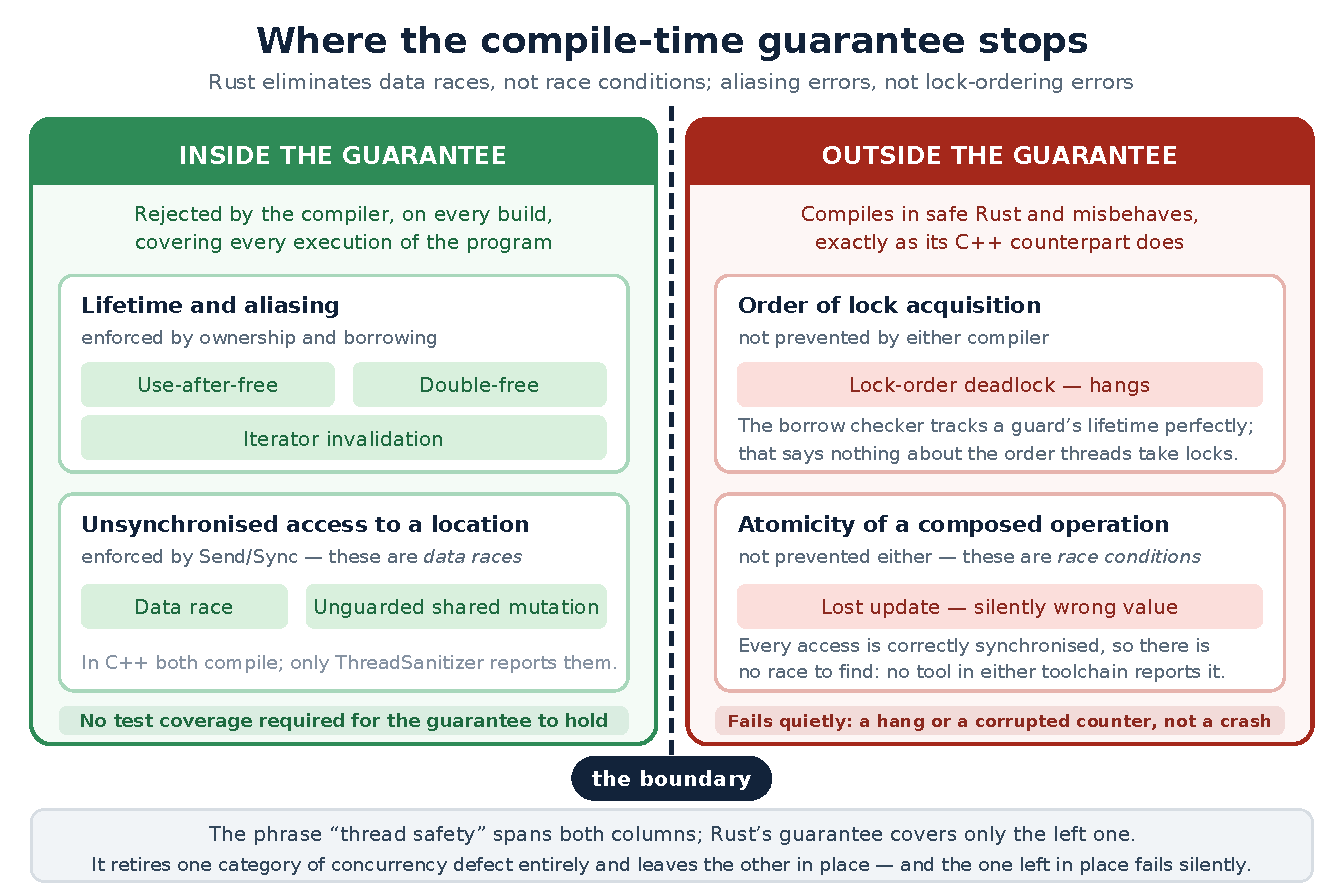
\includegraphics[width=0.78\linewidth]{diagrams/pdf/17_guarantee_boundary.pdf}
\caption[Where Rust's compile-time guarantee stops]{Where the compile-time guarantee stops. On
the left are the classes safe Rust rejects outright, grouped by the \emph{mechanism} that rejects
them rather than by defect family: ownership and borrowing for lifetime and aliasing errors, which
is why iterator invalidation sits with them, and the \texttt{Send}/\texttt{Sync} discipline for
unsynchronised access to a location. On the right are the classes the catalogue included to find
the edge, which neither compiler prevents. The diagram names one class per mechanism and is not
the catalogue, which Table~\ref{tab:defectmap} lists in full: the use-after-move belongs with the
ownership cases on the left and the shared thread-unsafe handle with the
\texttt{Send}/\texttt{Sync} ones, while the leak, the release-build overflow, the worker-failure
case, the seam double-free and the forgotten guard sit alongside the two on the right. The phrase
``thread safety'' spans both sides of the line, and the guarantee covers only the left. The line
itself moves once more than the diagram can show, because a program that writes \texttt{unsafe}
crosses it voluntarily.\label{fig:boundary}}
\end{figure}

\paragraph{RQ3 (overhead).} The answer splits by resource, and the splits do not all point the
same way. On memory there is a penalty: the Rust build carries a few MiB more peak resident set
and keeps that sign under both allocators. Two things make it credible beyond the $p$-value. Peak
RSS is a run-level maximum and not a tail statistic, so the scheduling jitter that destroys the
p99 does not touch it, and it reproduces on a second machine with a different compiler
(Section~\ref{sec:baremetal}), which no other timing-adjacent result here can claim. The useful
way to size it is against the allocator's own effect, and that comparison is the part which does
\emph{not} travel. The two are of comparable size on the reported host and on the second
bare-metal one, while on the virtualised host the allocator's was an order of magnitude larger,
because the allocator effect shrank by more than ten times across the change of machine and the
language effect did not move. The language effect replicates and its ratio to the allocator's does
not, so whether a few MiB of language choice is more or less than the allocator choice is a
question about the machine.

On CPU the answer depends on the load, and that dependence is the finding. Below saturation Rust
draws slightly \emph{less} under both allocators, and past saturation the sign flips and the
magnitude grows (Section~\ref{sec:overload}), so a single number for ``the CPU cost of Rust's
safety model'' would average two regimes behaving in opposite directions, and neither figure is
the safety model in any case. Throughput splits the same way: below saturation there is nothing to
measure, because achieved throughput tracks offered load by construction, and above it sits the
largest effect in the study.

Three things bound what the memory penalty licenses. It is a fixed cost rather than a per-context
one, so its share of a deployment's footprint falls as the deployment grows. It is located
\emph{outside} the allocator by the allocator's own accounting, since the Rust build holds less
live data and fewer resident bytes inside \texttt{jemalloc} and still peaks $\BmJeRssDelta$~MiB
higher (Section~\ref{sec:hostcompare}), which makes it a one-off charge per process for the
standard library and the runtime rather than a tax on the work. And nothing here isolates bounds
checking or ownership-driven copying as the cause: the mechanisms the literature has
localised~\cite{zhang2022runtime,harris2023morello} are candidates to test, not conclusions to
import. Adopting Rust here costs a few megabytes of fixed footprint per process and buys a faster
core operation (Section~\ref{sec:budget}) that this workload's structure never turns into
throughput below saturation, and that turns into a deficit above it.

The sign of that result is worth defending, because one of the closest prior works reports the
opposite sign while two others agree with it. A second Ericsson-hosted study of RAN node
management software found Rust's peak memory usage generally higher than
C's~\cite{olsson2023ranmgmt}, and a matched pair of user-space device drivers outside telecom put
the Rust version's footprint about 29\% above the C version's~\cite{sundvisson2026drivers}.
Neither separates the allocator from the language, the distinction Section~\ref{sec:resources}
rests on, so they support the direction and not the split.

The disagreement is more instructive. Karlb\"ack and Or\"o measure peak resident set on a RAN
workload and find Rust the \emph{lowest} of three languages and C++ the highest, with the gap
widening as concurrency rises, a pattern they call surprising and attribute tentatively to the
initial stack size of the green threads~\cite{karlback2021ran}. The two findings are compatible
once it is clear they measure different quantities. Their C++ runs on Boost.Fibers, which
allocates a stack per fiber, so ten thousand concurrent sequences cost ten thousand stacks, while
their Rust runs on Tokio, where a task is a heap-allocated future of a few hundred bytes. Their
figures capture the per-context cost of the concurrency runtime, which is why it grows with the
number of contexts. The design measured here has no green threads on either side, and a fixed
thread-per-shard pool leaves no per-context allocation to differ, so what remains is a fixed
footprint constant in the number of UEs. Their disagreement is between two concurrency runtimes
and not between two languages, which is as direct a demonstration as the literature offers of why
this study holds the concurrency model fixed. It also sharpens the caveat on the present number,
which licenses nothing about Rust's memory behaviour under a task-per-UE design.

\paragraph{RQ4 (migration).} Incremental adoption is technically cheap. A C++ host can call an
unmodified Rust core across a thin C-ABI seam whose cost on a real operation is bounded at
$\FfiOpBoundPct\%$, and all \texttt{unsafe} stays inside the seam. That bound comes from the
matched comparison of Section~\ref{sec:migrationresults} and not from setting an empty crossing
against a full round-trip, which are different experiments: on this host a single unpaired pass of
each was enough to flip the apparent ordering. The dominant cost is human rather than machine,
designing a C-compatible surface and, as the adoption studies
report~\cite{fulton2021adopting,crichton2024learning}, climbing Rust's learning curve. That makes
migration risk organisational and not a performance concern, and the two largest documented
adoptions into existing C and C++ codebases report the same ordering of
costs~\cite{li2026rustlinux,fan2026android}.

One boundary has to be drawn explicitly, because the natural reading overstates it. ``All
\texttt{unsafe} confined to the seam'' is a claim about what the compiler verifies, true as
measured, with no \texttt{unsafe} in the core crate and every raw-pointer operation in
$\FfiUnsafeFns$ reviewable functions. It is not a claim that the core is protected at run time.
Host and component share an address space, and a memory error on the C++ side can corrupt
Rust-owned data however carefully the Rust side was checked, which is why the remedies proposed in
the literature isolate the two heaps with hardware support instead of relying on interface
discipline~\cite{rivera2021galeed,kirth2022pkrusafe}, and why the defect classes arising at such
boundaries have been catalogued in their own right~\cite{li2022crosslang}. A migration of this
shape buys a component that stops \emph{contributing} new memory-safety defects while it stays
exposed to those of the host, which is a reason to sequence a migration so that the components
sharing the most mutable state cross over together.

The three axes measured beyond the seam complicate two folk versions of the same conclusion. Build
time survives only in the aggregate: the full build does cost $\BuildAllCpuRatio$ times the CPU,
but $\BuildDepShareCpu\%$ of that is third-party code, so the project's own source compiles for
$\BuildAllFirstPartyCpuRatio$ times what \texttt{g++} spends on its equivalent, and an
organisation worried about build time should look at its dependency budget before its compiler.
The edit-compile loop is where C++ genuinely leads, unevenly, its advantage holding for edits
inside a translation unit and reversing for edits to a widely included header. Binary size behaves
worse than an argument would predict, since the $\FootShippedRatio\times$ figure that gets quoted
compares two linkage policies and the ordering depends on which policy is held. The axis that
matters most for a regulated codebase has the cleanest answer: the component compared here
resolves no third-party code and contains no \texttt{unsafe}, so the transitive-dependency
argument does not reach the artefact under discussion.

\section{Revisiting the hypotheses}\label{sec:hypotheses}
Section~\ref{sec:rqs} committed to three hypotheses before any measurement was taken. Stating
their disposition explicitly is what distinguishes a test from a description.

\begin{description}
  \item[H1: supported below saturation, refuted above it.]
        The hypothesis had two parts: that the languages are performance-equivalent below
        saturation, and that any difference is confined to the far tail. The first is supported.
        The second is refuted, and not in the direction the wording anticipated, for the reasons
        Section~\ref{sec:rqdiscussion} gives. The largest difference the study found lies in
        overload, which H1 did not consider at all, so the hypothesis as written would have led
        the campaign to look in the wrong place. The result was found because the sweep was pushed
        past saturation on methodological grounds rather than in expectation of it. The clause H1
        did name is half right. For most of this study the far tail could not be resolved at all,
        so that part was untestable rather than refuted. It is resolved now, in Rust's favour, at
        loads where the median difference is about a microsecond on an operation of
        $\PFiftyMedian\,\mu$s, and a second bare-metal campaign agrees on the direction
        (Section~\ref{sec:hostcompare}). H1 was right that the far tail is where a
        below-saturation difference would show up, and wrong that it is the only place any
        difference shows up. A second disposition is that the hypothesis is not well posed.
        ``Performance-equivalent'' was written as though it named one quantity, where
        Section~\ref{sec:budget} shows it names at least three: the delivered operation below
        saturation, the code the compilers emit, and sustained work under overload. Those three do
        not move together.
  \item[H2: supported in its precise form, refuted in its loose one.] The hypothesis was
        that safe Rust prevents at compile time ``the memory-safety and concurrency defect
        classes that C++ leaves to best-effort detection''. For the seven injected classes of
        that kind it holds without exception. The fault-injection study still refutes the broader
        reading the wording invites: the seven boundary classes are exactly the sort C++ leaves to
        best-effort detection, safe Rust does not prevent them either, and on the leak and the
        release-build overflow the C++ tooling is the one that reports. H2 is therefore accepted
        for memory safety and data-race freedom, and rejected for concurrency correctness at
        large. It also carries an unstated precondition the seam case makes explicit: the
        hypothesis is about \emph{safe} Rust, and the same class it rules out returns as soon as a
        program writes \texttt{unsafe}. The second reading is the one practitioners tend to
        assume.
  \item[H3: supported, and tested the right way on the second attempt.] The hypothesis was
        that interoperability cost is negligible against the operations invoked. Measured
        directly (Section~\ref{sec:migrationresults}), no cost is detected and any per-operation
        tax is bounded at $\FfiOpBoundPct\%$. What supports the hypothesis is the bound and not
        the failure to detect a difference. The first version of this measurement set an empty
        crossing against a full round-trip and inferred the answer, comparing two different
        experiments, which would have given the right conclusion for the wrong reason. The
        accompanying claim, that the real cost is engineering effort, is supported structurally
        and not statistically: the seam is small and mechanical, but designing its C-compatible
        surface was the part of the prototype that took actual design decisions.
\end{description}

\section{Engineering guidelines for incremental adoption}
\label{sec:guidelines}
Appendix~\ref{appendix:guidelines} records seven guidelines in the order a first migration would
run them, each tied to the finding that supports it and to the limit of that support. A guideline
quoted without its limit is how the RQ2 result becomes ``the migrated component is safe'' and the
RQ4 result becomes ``migration is cheap'', and this study establishes neither. Two belong in the
running text because the study arrived at them late. An end-to-end request/response measurement of
this design is $\BudgetCoreShareMax\%$ language and the rest scheduler
(Section~\ref{sec:budget}), so below saturation it returns ``no difference'' between almost any
two competent implementations, and a vendor running its own comparison should budget for the
end-to-end measurement, which says what a deployment will feel, and the component measurement,
which says what the language is doing. Every conclusion drawn while the sweep stopped at nominal
load was a null, correct at that operating point and silent about the one where the two
implementations differ by $\OverloadThrRatio\times$ (Section~\ref{sec:overload}). The reusable
artifact is the benchmarking framework and not its current output.

\section{Related work}\label{sec:relatedwork}
Chapter~\ref{chapter:background} set out the ground this work stands on in four strands, and
Appendix~\ref{appendix:search} records the position each leaves this thesis in. The studies the
thesis has to answer to are treated here.

Four systems studies come closest in method, though not in domain, because they too build the
same component twice and attribute the difference: inter-process communication (IPC) mechanisms
for one network function~\cite{li2021ipc}, RedLeaf against purpose-built C
baselines~\cite{narayanan2020redleaf}, a concurrent translation of the Stanford Transactional
Applications for Multi-Processing (STAMP) benchmarks that is the closest published match to this
design~\cite{suchert2023stamp}, and a kernel User Datagram Protocol (UDP) tunnelling
driver~\cite{gonzalez2023rustudp}. That last reports Rust slower by 0.19\% at $p = 1.5 \times
10^{-15}$, a difference overwhelming in statistical terms and negligible in operational ones, and
keeping those two apart is what the pre-committed interval-versus-$p$ rule of
Section~\ref{sec:stats} exists to do. None of the four measures past saturation.

Five master's theses, all carried out at Ericsson, are the closest prior work by domain. None is
peer-reviewed and none is indexed by any citation database, so they are cited as the record of
what a vendor has attempted rather than as established results.

Karlb\"ack and Or\"o's control is the confound this study is built to remove. They ``aimed for
providing the best solution in each language, instead of trying to make the code as identical as
possible between the languages''~\cite{karlback2021ran}, so the concurrency runtime varies with
the language and no measured difference can be divided between the two.
Section~\ref{sec:rqdiscussion} returns to this where their resource results and the ones reported
here have opposite signs. Olsson's later management-software comparison agrees with this study on
two of three findings, including that resource result, and does not report percentiles or drive
the software past capacity~\cite{olsson2023ranmgmt}. Olsson and Stenstr\"om's asynchronous Rust at
a fifth to a half of DPDK's throughput is the sharpest illustration of why the model has to be
held fixed: an effect of two to five times is not the scale at which code generation
operates~\cite{olsson2023asyncpackets}.

Arvidsson and Kaller are the most direct challenge to the expectation this thesis set out with.
Across five asynchronous frameworks on 5G control-plane procedures, Boost.Fibers shows the lowest
latency at every load, and while the Rust runtimes track it at the median, their 99th percentile
rises more steeply beyond a certain request rate~\cite{arvidsson2025async}. That is a tail
divergence in the right domain and it would be dishonest to omit it. It is also a comparison in
which the runtime co-varies with the language. \v{S}koudlil et al.\ report that Tokio is
``designed to maximize throughput rather than time determinism'', and that restructuring onto
prioritised threads yields response times matching classical
analysis~\cite{skoudlil2025asyncrust}, priority scheduling being something an asynchronous Rust
runtime has to be given by a library~\cite{zhuang2026flowprioritize}. The two studies are
complementary: theirs establishes that a tail difference is observable in this domain, and this
one is built to determine whether the language causes it.

Emberg and Wadsten are the closest of the five in method, a matched pair with an FFI seam, a
statistical comparison and an effort measurement, two years earlier~\cite{emberg2023asn1}. Three
differences carry the gap: the object is a stateless transformation, the measurements are taken at
a fixed load, and the safety side is argued from interviews rather than a defect catalogue. Their
warning travels further than the comparison. Two benchmarking sessions reversed the verdict,
comparable after a code review and then Rust worse by 85--91\% after further optimisation, so a
single-author matched pair can be made to yield either answer. Section~\ref{sec:threats} treats
that as the principal threat to construct validity.

Two 2026 bachelor's theses from outside the vendor set apply parts of the method to smaller
objects: matched C and Rust user-space drivers, with a fixed memory overhead and no measurable
run-time cost~\cite{sundvisson2026drivers}, and a Common Weakness Enumeration (CWE) staging
study across C++, Rust and Python~\cite{andersson2026stdmemsafety}. Neither involves concurrency,
a telecom workload, or a load sweep.

Table~\ref{tab:vendortheses} sets this study beside the five directly. The earlier work is not
weaker, only aimed differently: four of the five measure a language together with the framework it
was written on, and the fifth measures a matched pair on a stateless object at a fixed load. The
verdicts in the last column then contradict one another in every direction, on peak memory, on
throughput and at the median, because no two of them hold the same things fixed. That is the
signature of a literature in which the independent variable is not controlled, and it is why this
thesis builds its object of study instead of finding one.

\begin{table}[tp]
\centering
\small
\caption[This study beside the five vendor theses]{This study beside the five vendor theses, all
carried out at Ericsson and none peer-reviewed. The rows are ordered by year. The last column
reports each study's own verdict in its own terms, which is why the entries do not line up: they
are answers to different questions, measured on different objects in different regimes. The
verdict recorded for this thesis is the one Section~\ref{sec:rqdiscussion} defends, including the
part that runs against its own expectation. Figure~\ref{fig:gapmap} places the same five studies on
the axes of the gap instead, alongside the peer-reviewed
literature.\label{tab:vendortheses}}
\renewcommand{\arraystretch}{1.2}
\begin{tabular}{@{}R{0.18\linewidth} R{0.25\linewidth} R{0.20\linewidth} R{0.26\linewidth}@{}}
\hline\hline
Study & Object measured & Regime reported & Reported verdict on Rust \\
\hline
Karlb\"ack \& Or\"o, 2021~\cite{karlback2021ran} &
RAN applications on x86 and Arm, one idiomatic implementation per language &
Runtime and resource use at the loads exercised &
C++ preferred where performance is critical. Rust's peak memory the lowest of the three
languages \\
Olsson, 2023~\cite{olsson2023ranmgmt} &
RAN node management software, Rust against C &
Execution time and peak memory &
Speed on par with or better than C, peak memory higher, safety materially improved \\
Olsson \& Stenstr\"om, 2023~\cite{olsson2023asyncpackets} &
Packet processing: asynchronous Rust on Glommio against DPDK Eventdev in C &
Throughput and latency against core count &
20--50\% of DPDK's throughput with far worse latency. Asynchronous Rust judged not currently
viable \\
Emberg \& Wadsten, 2023~\cite{emberg2023asn1} &
An {ASN.1} decompiler built twice, the Rust side reaching C++ through a C wrapper &
Execution time in two benchmarking sessions &
Comparable in the first session, 85--91\% worse in the second. Preferred in practice on
non-performance grounds \\
Arvidsson \& Kaller, 2025~\cite{arvidsson2025async} &
5G control-plane procedures across five asynchronous frameworks &
Median and 99th percentile across a load sweep &
Median tracks C++. The 99th percentile rises more steeply past a threshold request rate \\
\hline
This thesis, 2026 &
A UE Context Management service built twice from one frozen specification, with the concurrency
model, allocator and build settings fixed &
Median, p99, p99.9, p99.99 and maximum across a sweep to and beyond saturation, on a bare-metal
host and reproduced at a second shard count &
Equivalent at the median below saturation. The far tail there resolves and favours Rust. Past
saturation \OverloadSustainedFaster{} sustains
$\OverloadThrRatio\times$ the throughput of \OverloadSustainedSlower{} \\
\hline
\end{tabular}
\end{table}

Section~\ref{sec:gap} recorded that all five come from one vendor. Findings such as ``C++ remains
the choice where performance is critical'' and ``asynchronous Rust is not currently viable''
describe particular software on particular infrastructure, and repetition inside one organisation
does not establish their generality. The specification, both implementations and the harness are
published with this thesis so that an independent organisation can check the answer given here.

Not all of this evidence points the same way, and the qualifying findings are taken as seriously
as the favourable ones. Even the positive networking result records a real cost: the idiomatic
Rust driver issues substantially more instructions per packet than its C reference and is
measurably slower in absolute terms, its safety checks absorbed by out-of-order execution rather
than literally free~\cite{emmerich2019drivers}. Idiomatic safe Rust implementations of the STAMP
transactional benchmarks run slower than both the C originals and machine-transpiled
Rust~\cite{suchert2023stamp}, a general study of Rust against C reports it significantly slower in
some cases~\cite{okawa2024ruststudy}, and the largest study of Rust inside an existing C codebase
finds that Rust's safety features introduce runtime overhead and development complexity when they
are not carefully managed~\cite{li2026rustlinux}. The evidence does not run one way, though. Safe
low-level code without run-time overhead has been demonstrated for network device drivers, the
same class of program as Emmerich's, when the safety obligations are discharged through type
invariants rather than checks~\cite{pirelli2023safelowlevel}. The ``zero-cost''
framing~\cite{balasubramanian2017rust} is therefore best read as neither established nor refuted
in general, but as a property of a particular program on a particular workload, which is why tail
behaviour must be measured on the target workload and not assumed. The safety story is likewise
not absolute: empirical studies of real-world Rust find that memory- and thread-safety bugs still
occur in practice, with blocking bugs and misused synchronisation among
them~\cite{qin2020rust,qin2024safety}, and that a substantial fraction of the ecosystem cannot be
fully statically checked, because \texttt{unsafe} propagates through dependency
chains~\cite{evans2020rust}. These qualifications do not overturn the case for Rust. They motivate
measuring predictability and defect prevention directly on the subsystem instead of importing
general-purpose, average-case conclusions, and keeping the safety-critical core
\texttt{unsafe}-free so that the dependency-propagation caveat does not apply to it.

Three axes separate this thesis from all of it: Whether the comparison controls for design by
building both systems from one specification, whether it reports tail behaviour under overload
instead of average-case performance, and whether it measures the cost of adoption instead of
describing it. None is unoccupied on its own, as the matched
implementations~\cite{emmerich2019drivers,li2021ipc,narayanan2020redleaf,suchert2023stamp,gonzalez2023rustudp,pirelli2023safelowlevel,emberg2023asn1},
the percentile sweep stopping at a latency requirement~\cite{arvidsson2025async} and the effort
measurements~\cite{karlback2021ran,fulton2021adopting} all show. No prior study combines the
three for a stateful, concurrent control-plane workload, and that is the narrower gap this work
occupies.

\section{Threats to validity and mitigations}\label{sec:threats}
Every conclusion here attributes a difference to the implementation language, so the credibility
of the study rests on the controls that hold everything else equal and on an honest account of
where those controls stop. Table~\ref{tab:threats} maps the threats by the kind of inference each
endangers, so the remaining risks can be read as a set rather than gathered from the prose. Three
are load-bearing. The study cannot rule out single-author skill asymmetry. Its end-to-end
instrument is the wrong one for part of what RQ1 and RQ3 ask. And its strongest single finding,
the overload divergence, rests on an attribution it did not measure directly.

\begin{table}[tp]
\centering
\small
\caption[Threats to validity, their mitigations, and what remains]{Threats to validity by the kind of inference each endangers, the control applied, and
what that control leaves behind. Only the last column holds live risks. Two of the controls arrived
with the host comparison of Section~\ref{sec:hostcompare}.\label{tab:threats}}
% Slightly opened row height on the densest table in the thesis, which overruns the
% page without it. The \singlespacing is redundant now that the body is single-spaced
% too, but it is kept because it reselects the current size, which is why it has to
% come before \footnotesize rather than after it.
\singlespacing
\footnotesize
% 1.15 rather than 1.25, measured 27 Aug 2026. The fifteenth row took the table
% 79pt past its page; tightening four cells recovered half of that and this
% recovered the rest. The table sits within a few points of a full page, so
% measure after any row edit rather than assuming there is slack.
\renewcommand{\arraystretch}{1.15}
\begin{tabular}{@{}R{0.23\linewidth} R{0.35\linewidth} R{0.32\linewidth}@{}}
\hline\hline
Threat & Control applied & What remains \\
\hline
\multicolumn{3}{@{}l}{\emph{Internal: is the language really the only difference?}} \\
Implementation bias between the two versions & Frozen specification, shared allocator and optimisation level, pinned hash functions, forced-idiom log, transcript-level parity testing & Single-author skill asymmetry. Parity bounds behaviour, not performance \\
\hline
\multicolumn{3}{@{}l}{\emph{Construct: do the metrics measure what the questions ask?}} \\
The sweep measures the design, not the language & The operation is measured apart from the handoff and both are reported (\S\ref{sec:budget}) & One operation on one data structure is narrower than the sweep it supplements \\
The overload result is attributed but not localised & Narrowed to two entries in the forced-idiom log (\S\ref{sec:overload}), and the contended-primitive microbenchmark rules those two out alone (\S\ref{sec:contention}) & The full handoff path under load still includes variant dispatch and larger requests on the C++ side \\
A defect catalogue is a sample the author chose & Seven classes drawn from outside the guarantee, with expectations recorded in advance & Fourteen programs remain fourteen programs \\
RQ3 captures resource cost, and its origin outside the allocator & The allocator's own accounting, on two bare-metal hosts (\S\ref{sec:hostcompare}) & No call site: the profiling build reverses the sign of the effect (\S\ref{sec:hostcompare}) \\
RQ4 measures the seam, not the safety of the whole & The distinction is stated wherever the result is quoted & One address space: a compile-time property of the Rust side bounds nothing at run time \\
\hline
\multicolumn{3}{@{}l}{\emph{Conclusion: are the differences real or noise?}} \\
Run-to-run non-determinism & \NRepeats{} interleaved repeats, bootstrap intervals, exact paired permutation test, Holm correction, floors quoted & Pairing cancels only what a block shared, which is why the far tail needed a quieter machine rather than more repeats \\
A corrected $p$-value that does not replicate & The allocator control runs every comparison twice. Replication is followed over the $p$-value & It has cost a result before and would again. Every comparison now replicates \\
A contaminated run defeating a mean-based statistic & The reading rule of \S\ref{sec:stats}, fixed in advance, plus the per-repeat agreement count & Nothing here: the bimodality behind the rule was the previous machine's. The rule is kept anyway \\
An operating point chosen after seeing the data & Both tested operating points are fixed in \S\ref{sec:stats} before the results & The saturation-limit gap (\S\ref{sec:perfresults}) is therefore descriptive, and the one comparison with no $p$-value \\
\hline
\multicolumn{3}{@{}l}{\emph{External: how far do the results travel?}} \\
One subsystem, one workload & RQ2 rests on the compilers, RQ4 on the compilers, the C ABI and the dependency graph & The performance results do not travel, the overload result least of all. RQ4's build seconds describe one machine, its ratio does not \\
One measurement host & Bare metal, no hypervisor, fixed governor, tickless pinned cores, and the same design re-measured on two further machines (\S\ref{sec:hostcompare}) & No \texttt{isolcpus} (\S\ref{sec:testbed}). Each comparison campaign changes something besides the machine, so both corroborate rather than replace \\
\hline
\end{tabular}
\end{table}

\paragraph{Internal validity: is the language really the only difference?}
The central threat is implementation bias between the two versions, mitigated structurally by the
controlled-variable strategy of Table~\ref{tab:controls} and the transcript-level parity testing
of Section~\ref{sec:parity}. What those leave behind is single-author skill asymmetry: one person
wrote both implementations and is not equally expert in both. That the threat is real and not
merely conceivable is documented in the same industry, by the two benchmarking sessions of Emberg
and Wadsten that reversed their own verdict~\cite{emberg2023asn1}, where one matched pair
supported two different conclusions depending on where the optimisation effort landed. The
controls here are chosen against that failure mode. The specification is frozen before either
implementation is written rather than negotiated between them, the optimisation level and
allocator are matched rather than tuned per side, and forced divergences are logged rather than
resolved in whichever direction the author finds easier. None of that reduces the remaining risk
to zero. It makes that risk visible, which is why the forced-idiom log is a deliverable and not an
appendix.

\paragraph{Construct validity: do the metrics measure what the questions ask?}
RQ1 is answered with high percentiles and the maximum instead of the mean, the standard way of
measuring predictability in this literature~\cite{dean2013tail}. Two risks remain. The metric list
was narrowed while the instrumentation for inter-operation jitter and p99.99 did not yet exist,
and both are now collected and reported, so the narrowing has been undone rather than merely
acknowledged. Jitter is the one metric the question still does not name, and it is reported
descriptively for that reason rather than tested. And p99.9 on a synthetic workload is not the
same quantity as a missed procedure deadline in a live network.

A second and larger construct gap in RQ1 was found rather than anticipated. The end-to-end latency
the sweep reports is $\BudgetCoreShareMax\%$ operation and the rest cross-thread handoff
(Section~\ref{sec:budget}), so it measures the delivered cost of the design faithfully and the
cost of the language barely at all. Which of those RQ1 asks about depends on the reader: a vendor
sizing a node wants the first, a language comparison the second. The study reports both and keeps
them apart, but the question as originally worded did not tell them apart. Two remedies are
applied and no amount of statistical care substitutes for either. The operation is measured apart
from the handoff, and the sweep is pushed into the regime where the design stops absorbing the
difference. What remains is that a microbenchmark of one operation is a narrower object than the
sweep it supplements.

The remaining three are stated in Table~\ref{tab:threats}. RQ2's catalogue is fourteen
programs, two of which returned the opposite of the expected conclusion. RQ3 locates the
resident-set difference outside the allocator (Table~\ref{tab:resident}) and cannot name a call
site, because the profiling build reverses the sign of the effect. The mechanisms most likely
responsible have been isolated elsewhere~\cite{zhang2022runtime,harris2023morello}. RQ4
measures the seam and not the safety of the composed system: host and component share an address
space~\cite{rivera2021galeed,kirth2022pkrusafe}.

\paragraph{Conclusion validity: are the differences real or noise?}
The statistical treatment is set out in Section~\ref{sec:stats} and its outcomes in
Table~\ref{tab:significance}. The repeat count is chosen so that the design is not the binding
constraint: an exact test on \NRepeats{} pairs floors at $\MinAttainableP$, and at
$\CorrectedFloor$ after correcting \NTests{} comparisons, so a null here reflects the data rather
than the arithmetic. An earlier pass at seven repeats did not have that property, and its
corrected floor above $0.05$ made every null in the table uninterpretable.

Three limitations remain. First, one property of the host is short of the protocol on purpose. The
pinned cores are not isolated from the scheduler with \texttt{isolcpus}, because isolating them
also removes them from every scheduling domain, and the benchmark pins its threads to a range and
relies on the kernel to spread them: an isolated set collapses all of them onto one core, which is
not a subtle failure but is an invisible one, since every individual record still looks plausible.
What that costs is a residue of scheduler interference on the pinned cores, bounded and not
eliminated by tickless operation on those cores, a fixed governor with boost off, and no
hypervisor beneath them (Section~\ref{sec:testbed}). The reading rule fixed in
Section~\ref{sec:stats} is aimed at exactly this residue: peak RSS, CPU and sustained throughput
are run-level summaries and come through cleanly, while the tail percentiles are computed from
precisely the operations any interference falls on, and their intervals are not read as findings
for that reason. On this host the rule changes no verdict, which is a fact about the machine and
not a reason to withdraw the rule. It is also why the overload comparison is made on throughput
and not on latency.

Second, a corrected $p$-value below $0.05$ is necessary here and visibly not enough. On an earlier
campaign, before the two \texttt{jemalloc} builds were held to one configuration, CPU utilisation
cleared Holm under one allocator and reversed sign under the other, and no threshold would have
caught that. The opposite case appeared on the earlier host, where peak resident set size under
\texttt{jemalloc} showed an interval far from zero against a $p$-value near unity, which a handful
of runs reporting a resident set $\GuestRssLowRunOffset$~MiB low are enough to produce. That row
was read from its interval under the rule of Section~\ref{sec:stats}. The bimodality belonged to
that machine (Section~\ref{sec:hostcompare}), and the rule is retained because that is what a
pre-commitment means.

Third, the overload divergence is measured and replicated, and its mechanism is now tested and not
only argued. Isolated under the same pattern of \ContentionProducers{} producers, the bounded
queue and completion primitives do not reproduce the full-service ordering at significance
($p = \ContentionP$), which rules those two constructs out alone as the whole explanation even
though they are where the forced-idiom log predicted contention would matter. The cause is not
unknowable, and Section~\ref{sec:contention} names the candidates that remain on the C++ handoff
path.

\paragraph{External validity: how far do the results travel?}
The study covers one subsystem, one workload, one concurrency structure and one machine. The
safety and migration results (RQ2, RQ4) travel most easily, because they are properties of the
compilers and of the C ABI and not of this subsystem: any C++ codebase writing these defect
classes gets the same compile-time outcome, and any narrow, scalar-typed interface gets a
similarly cheap seam. Two of RQ4's adoption axes carry the same way, because a binary's size and a
dependency graph's shape follow from the toolchain. The third does not travel as an absolute,
because build seconds belong to the machine that measured them and what carries is the ratio
between two toolchains timed alternately. The build-time \emph{shape} is specific too: a two-file
C++ library and a single Rust crate are both small, and the incremental result in particular would
move on a codebase with a different header structure.

The performance results travel least. UECM was deliberately chosen to be small and partitionable,
and its shared-nothing design removes lock contention from the hot path, so a subsystem with
genuinely shared mutable state, deep call graphs, or heavy allocation churn could exercise the two
languages' abstraction and allocation costs quite differently. The workload is synthetic and
spec-justified, not replayed from production traffic, so its operation mix is plausible but
unvalidated. Nothing here speaks to PHY or L2 processing, to the data-heavy user plane, or to the
operational concerns (upgrade, observability, multi-tenancy) a production deployment would raise.

The defensible claim is therefore narrow and carries a condition. For stateful, concurrent,
partitionable control-plane services of this kind, and while they are meeting their offered load,
the language choice is not a performance decision. Once they are not meeting it, the language
choice is one. And the overload result is the least transferable finding in the study rather than
the most, because it depends on the queue bound, on one request being outstanding per producer,
and on two particular standard-library primitives. Extending either claim beyond this class means
rerunning the framework, which is why the framework and not the numbers is offered as the reusable
contribution.

A final limit on reach is temporal rather than structural, and it applies to the comparison
itself. One of the two objects being compared is moving. The C++ side is pinned to C++23 and to
the compiler versions recorded in Section~\ref{sec:testbed}, while the standards committee pursues
enforced safety profiles (Section~\ref{sec:cpplatency}). That qualifies nothing measured here,
because none of that work is standardised or generally implemented and the concurrency profile
that would reach the boundary classes of RQ2 comes after an initial set still to be
specified~\cite{vandevoorde2026profiles}. It does mean the RQ2 result describes these languages as
they stand and not permanently, which is why the catalogue is designed to be re-run against a
compiler that enforces such profiles.

\paragraph{Replication status: which findings stand alone.}
Internal replication is designed into the campaign, in \NRepeats{} interleaved repeats and in
every comparison being run twice under different allocators. External replication is uneven. Three
findings have published company: median equivalence below saturation, with matched pairs in three
settings putting safe Rust within single-digit percentages of its C or C++
counterpart~\cite{emmerich2019drivers,li2021ipc,gonzalez2023rustudp}, a cross-thread handoff
dominating the end-to-end cost~\cite{zhou2025oltp}, and most of RQ2's boundary classes, which the
literature already documents. Three stand alone. No study located by the protocol of
Appendix~\ref{appendix:search} reports a load-dependent reversal between the two languages, and the
one reporting the same shape attributes it to a runtime this design
excludes~\cite{arvidsson2025async}. None measures the two toolchains' build time with the
dependency tree separated from the project's own source. The per-operation bound on the seam has
no published counterpart. Peak resident set size sits between the two groups, with the sign found
here reported by two neighbouring theses and reversed by a
third~\cite{olsson2023ranmgmt,sundvisson2026drivers,karlback2021ran}. The overload divergence is
the largest single effect measured here and the finding with the least external corroboration.

\section{Ethical and professional reflection}
The study processes no personal, subscriber, or operator-confidential data. All traffic is
synthetic and the subsystem is modelled on production code rather than copied from it, so the
artifacts can be released openly. The \emph{use} of the study is a different matter, because a
language-selection recommendation in this domain is not a neutral technical output. Two
responsibilities follow. The first concerns over-claiming. A vendor could read the RQ2 result as
licence to describe a migrated component as ``safe'', and the boundary cases are why that reading
would be wrong: a deadlocked control plane is an outage, a silently lost counter update can
misinform a mobility decision, and nothing demonstrated here prevents either. Reporting the
boundary as prominently as the guarantee is a professional obligation, because the audience for
this work is making a decision that affects networks people depend on. The second concerns how far
the evidence reaches. Tail-latency numbers from any single machine are a narrower basis for a
production commitment than they look, which is why Table~\ref{tab:findings} carries an evidence
status per research question and why the earlier virtualised campaign is reported rather than
quietly discarded. A migration recommendation also carries organisational consequences, and the
cost moved from run time to human effort rather than disappearing.

